\chapter{Felhasználói dokumentáció}
\label{ch:user}

\section{Rövid leírás, fogalmak}

Különböző felhasználói fiók típusok magyarázata:

\begin{itemize}
  \item Kliens: Az edzők által edzett kliensek rendelkeznek ilyen típusú fiókkal. Egy kliensnek egyszerre egy edzője lehet.
  \item Edző: Ők állítják össze klienseik edzésterveit. Több klienssel is rendelkezhetnek.
  \item Adminisztrátor: Speciális adminisztrátori fiók, jogosultsággal rendelkezik a felhasználók listájának megtekintésére, valamint felhasználók törlésére. 
\end{itemize}

\bigskip

A weboldalon az \textbf{edzőknek} lehetőségük van \textbf{klienseik} számára ciklusokat\footnote[1]{A Ciklus egy összefoglaló név az olyan edzéstervekre, amelyek hetente ciklikusan ismétlődnek azonos gyakorlatokkal, több heten keresztül, hetenként eltérő nehézséggel} összeállítani. Egy ilyen \textbf{ciklus} több hétből állhat, hosszuk nem haladhatja meg a 6 hetet. Hetenként maximum 7 napra bonthatjuk az edzésterveket.
Egy adott napra több elvégzendő gyakorlatot rögzíthetünk, amelyeken a következő tényezőket állíthatjuk:
\begin{itemize}
  \item Gyakorlat neve
  \item Súly (weight)
  \item Szériák száma (series)
  \item Ismétlések száma (repetitions)
  \item Relatív nehézség (RPE)
\end{itemize}

\bigskip

Kliens felhasználók a saját névre szóló, edzőik által írt \textbf{ciklusaikat} elérik egy listában, az éppen aktív terveikben tudják módosítani az elvégzett gyakorlatok súly adatait, illetve a ténylegesen elvégzett \textbf{szériák}, \textbf{ismétlések} számát, illetve a tapasztalt \textbf{RPE} számot.

Kliensek edzőikkel kapcsolatba léphetnek egy beépített csevegő rendszer segítségével.

\section{Célközönség}

Az alkalmazás célközönsége azok, akik az erőemelés és más edzőtermi tevékenységek iránt érdeklődnek, és szeretnének fejlődni. Ide tartoznak azok, akik együttműködnének egy szakértő edzővel, valamint azok, akik edzői karriert szeretnének építeni a sportágban.

\section{Program használatához szükséges hardver- és szovtverkövetelmények}

A webapplikáció használatához egy friss verziójú böngészőprogramot futtatni képes hardverrel rendelkező eszközre van szükség, interneteléréssel.

A futtatáshoz ajánlott böngészők az alábbi felsorolt programok legfrissebb verziói, ezeken garantált az oldal helyes működése.
\begin{itemize}
  \item Google Chrome
  \item Mozilla Firefox
  \item Microsoft Edge
\end{itemize}

\bigskip

A futtatás során győződjünk meg arról, hogy böngészőprogramunkban engedélyezve van a JavaScript használata, mivel a felhasználói felület e technológiával van felépítve.

Az oldal reszponzív felhasználói felülettel rendelkezik, kisméretű kijelzőkön (minimum 375 pixel) is helyesen megjelenik, viszont a legjobb felhasználói élményhez legalább 1200 pixel széles kijelző ajánlott.

\section{Oldaltérkép}

\begin{figure}[H]
	\centering
	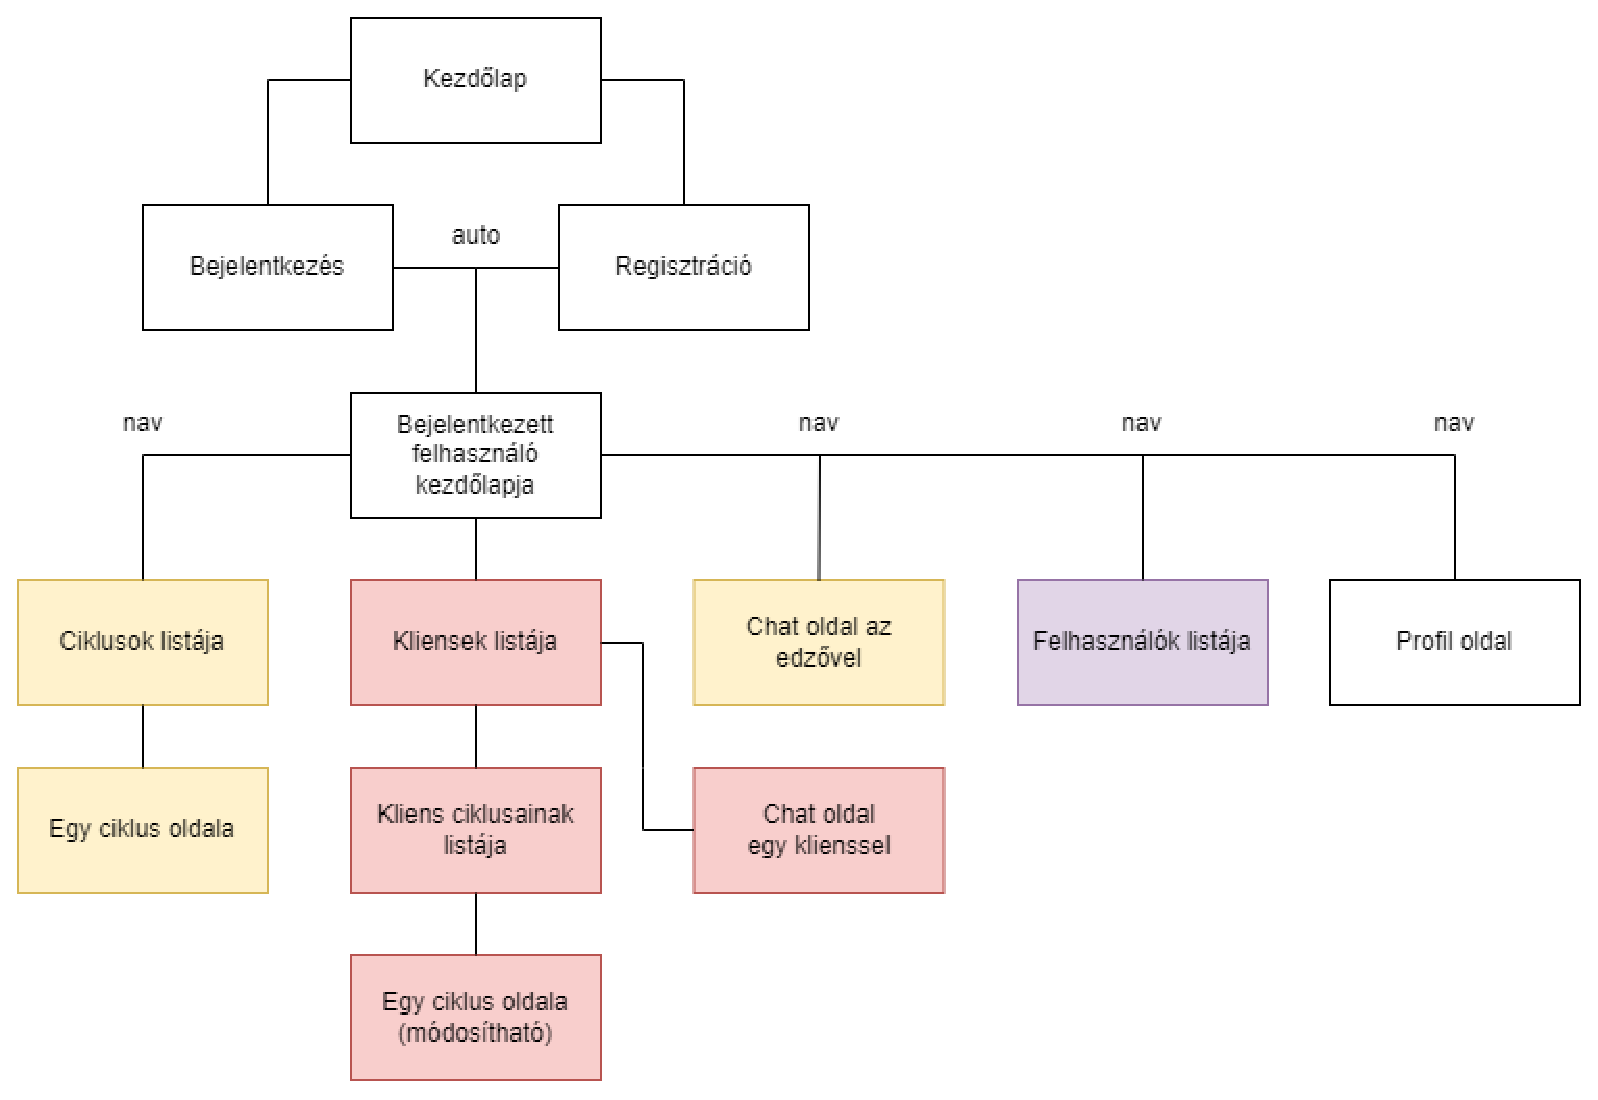
\includegraphics[width=1\linewidth]{oldalterkep}
	\caption{Oldaltérkép}
	\label{fig:oldalterkep}
\end{figure}

A \ref{fig:oldalterkep} ábrán a fehér kitöltésű mezők jelölik azokat az oldalakat, amelyeket bármilyen jogosultsággal rendelkező felhasználó képes elérni.
A citromsárga kitöltésű mezők a \textbf{kliens} jogosultsággal rendelkező felhasználó érheti el, a piros kitöltésűeket pedig \textbf{edző} típusú fiókkal lehetséges elérni.
A lila színű jelölés az \textbf{adminisztrátor} fiókok által elérhető oldalt jelöli.

A \textit{nav} kulcsszóval megjelölt útvonalak a navigációs menüből érhetőek el, az \textit{auto} kulcsszóval megjelöltek pedig automatikus átirányítás során, ha a felhasználó sikeresen bejelentkezett, vagy ha van bejelentkezett felhasználó eltárolva a készüléken.

\section{Weboldal funkcióinak bemutatása}

\subsection{Bevezetés}

Ebben az alfejezetben be fogom mutatni a webalkalmazás összes, felhasználók által elérhető oldalát, illetve kifejtem azok egyes funkcióit. Előszőr az összes, bejelentkezett felhasználó által elérhető oldalakat fogom bemutatni, majd rendre a \textbf{kliens}, \textbf{edző}, illetve \textbf{adminisztátor} jogosultságokkal elérhetőket.

\subsection{Kezdőlap}

\begin{figure}[H]
	\centering
	
\includegraphics[width=1\linewidth]{kezdolap}
	\caption{Kezdőlap}
	\label{fig:kezdolap}
\end{figure}

A \ref{fig:kezdolap} ábra mutatja a nem bejelentkezett felhasználóknak megjelenő kezdőlapot. A weboldal címe, rövid leírása látható. A jobb felső sarokban két gomb van elhejezve a felső navigációs sávban. A \textbf{Login} gomb megnyomásával a felhasználó a belejentkezési oldalra, a \textbf{Sign Up} gombra kattintással pedig a regisztrációs oldalra lesz átirányítva.

\subsection{Bejelentkezés}

\begin{figure}[H]
	\centering
	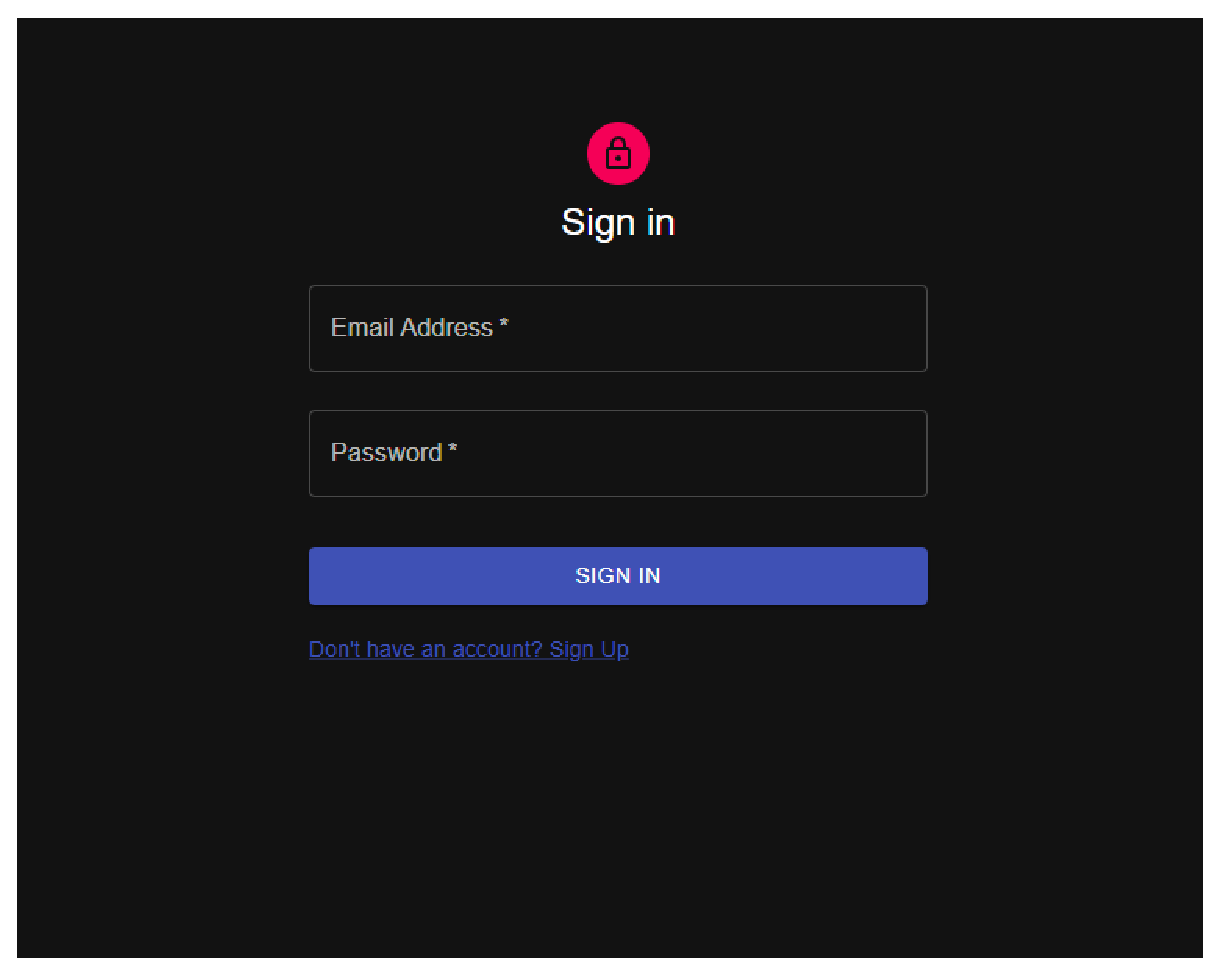
\includegraphics[width=1\linewidth]{login}
	\caption{Bejelentkezés}
	\label{fig:login}
\end{figure}

Az alkalmazásba funckiói eléréséhez előszőr be kell jelentkeznünk. Ezt a \ref{fig:login} ábrán látható oldalon tehetjük meg. A bejelentkezéshez meg kell adnunk a regisztrált fiókhoz tartozó email címet (Email Address) és jelszót (Password), majd a Sign In gomb megnyomásával a felhasználó a bejelentkezés után a kezdőlapra kerül, amennyiben helyes adatokat adott meg. Az oldal alján található link segítségével könnyedén át lehet kerülni a Regisztráció oldalra, amennyiben még nincs felhasználói fiókunk.

\subsection{Regisztráció}

\begin{figure}[H]
	\centering
	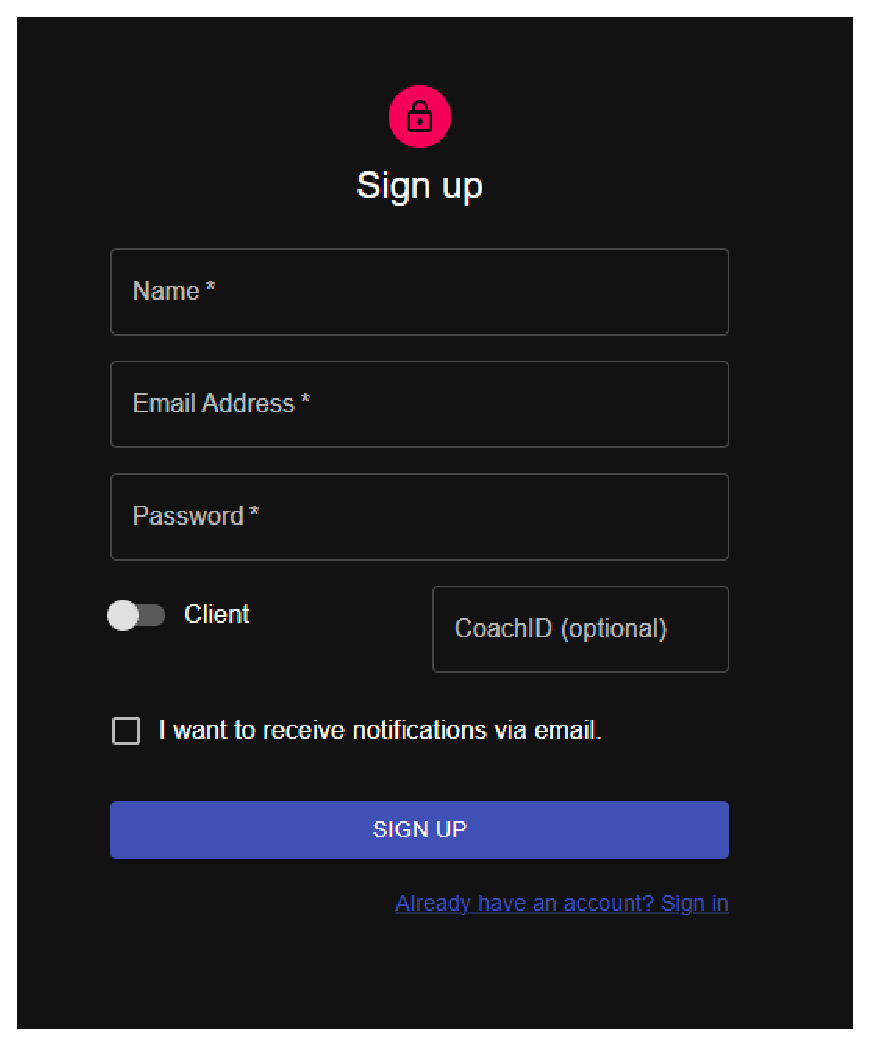
\includegraphics[width=0.6\linewidth]{register}
	\caption{Regisztráció}
	\label{fig:register}
\end{figure}

\begin{figure}[H]
	\centering
	
\includegraphics[width=0.6\linewidth]{registerslider}
	\caption{Regisztráció (edzői fiók)}
	\label{fig:registerslider}
\end{figure}

A felhasználói fiókunkat a \ref{fig:register} ábrán mutatott oldalon tudjuk létrehozni. Ezen az űrlapon ki kell töltenünk a fiókunk nevét (Name), ez fog megjelenni az alkalmazásban, mint felhasználónév. Meg kell adnunk egy email címet (Email Address), amelynek egy létező email címnek kell lennie. A jelszó (Password) mező kitöltése után van még lehetőségünk választani, hogy milyen típusú fiókot szeretnénk létrehozni. Kliens (Client) felhasználói fiók létrehozása esetén megadhatunk egy edző egyedi azonosítóját (CoachID), így regisztráció során is képesek vagyunk hozzárendelni fiókunkat egy edzőhöz. Opcionálisan be tudjuk kapcsolni az email értesítéseket (I want to receive notifications via email). Bekapcsolása után a megadott email címen keresztül értesülni fogunk a regisztráció sikerességéről. Az űrlap elküldése után visszakerülünk a kezdőlapra, amennyiben nem történt hiba az adatok megadásával. Az oldal alján látható egy link, ennek megnyomásával átkerülünk a Bejelentkezés oldalra.

\bigskip

Regisztrálni egy valós email címmel, jelszóval tudunk, illetve egy 20 karakterhosszt meg nem haladó felhasználónév megadásával.

\subsection{Kezdőlap (kliens)}

\begin{figure}[H]
	\centering
	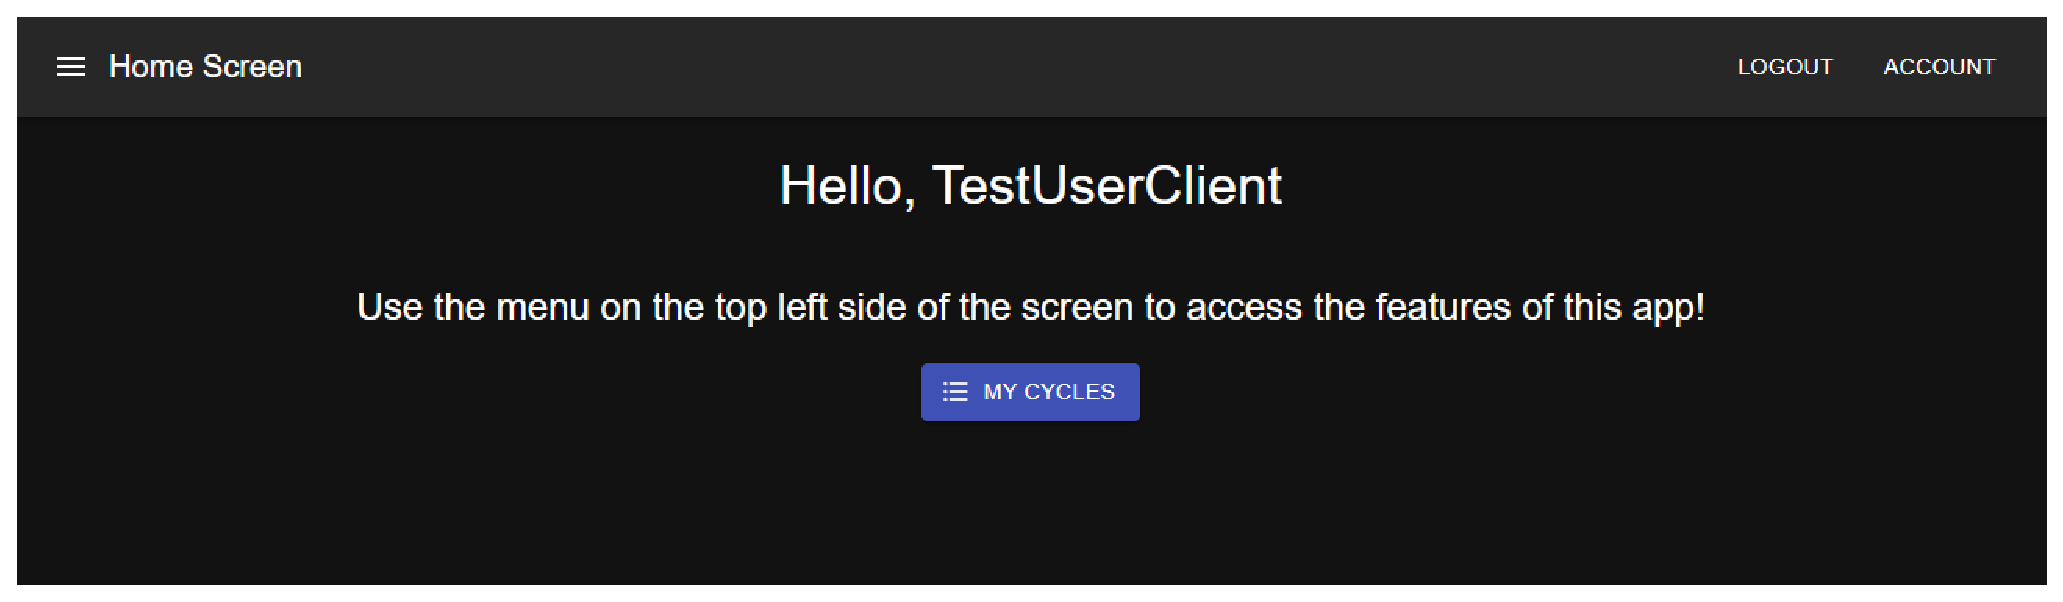
\includegraphics[width=1\linewidth]{kezdolapclient}
	\caption{Kezdőlap (kliens)}
	\label{fig:kezdolapclient}
\end{figure}

A \ref{fig:kezdolapclient} ábrán a Kezdőlap látató, ha a felhasználó kliens típusú fiókkal lép be az alkalmazásba. Az oldalon található egy gomb (My Cycles), amely a ciklusok listázó oldalára fogja átirányítani a felhasználót.

\subsection{Navigációs menü (kliens)}

\begin{figure}[H]
	\centering
	\includegraphics[width=1\linewidth]{navbarclient}
	\caption{Navigációs menü (kliens)}
	\label{fig:navbarclient}
\end{figure}

\begin{figure}[H]
	\centering
	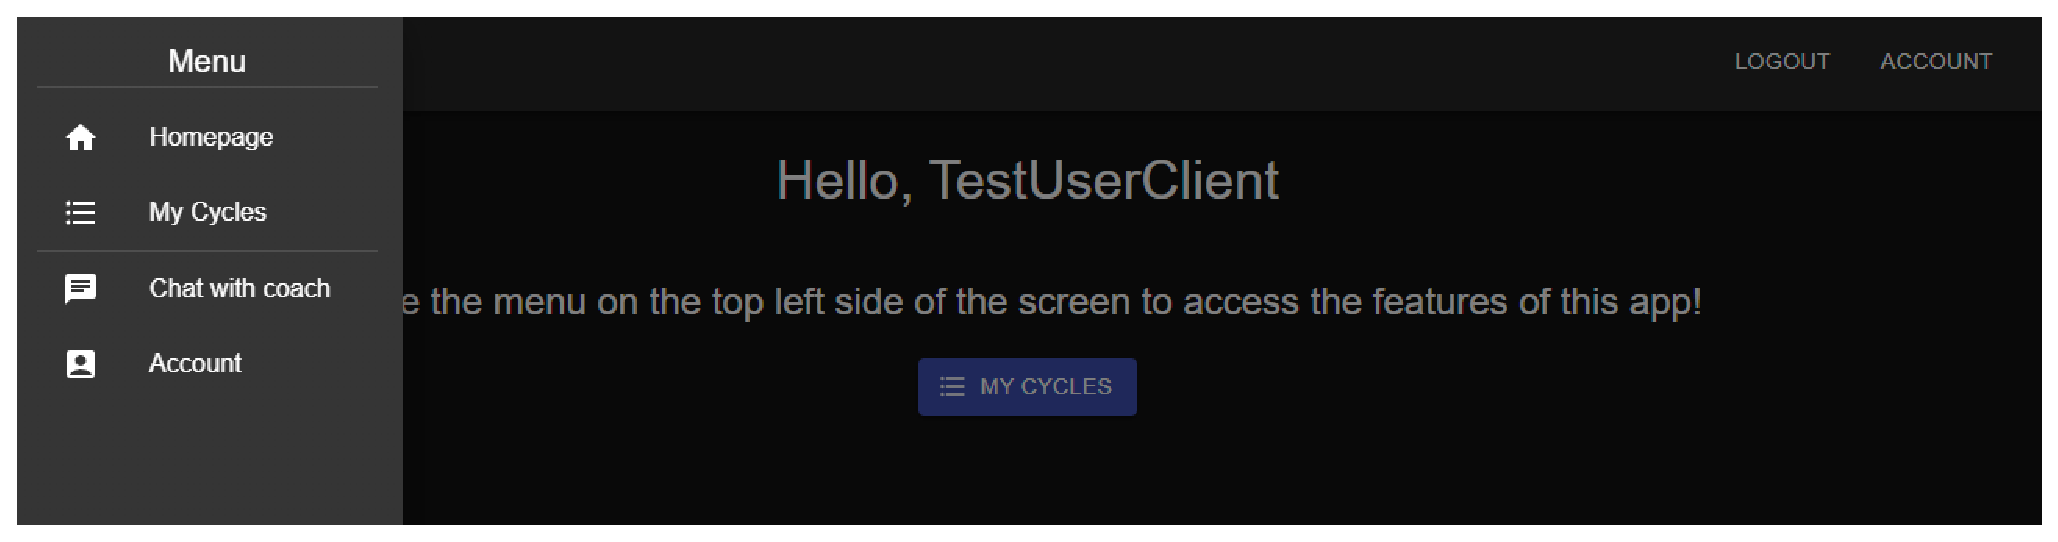
\includegraphics[width=1\linewidth]{navbarclienthascoach}
	\caption{Navigációs menü (kliens, rendelkezik edzővel)}
	\label{fig:navbarclienthascoach}
\end{figure}

A \ref{fig:navbarclient} ábrán a navigációs menü szerepel, kliens jogosultságokkal rendelkező fiókkal. A Homepage gombra kattintva visszakerülünk a kezdőlapra, a My Cycles gomb megnyomása után a ciklusok listázó oldalára kerülünk. \ref{fig:navbarclienthascoach} ábrán megfigyelhetjük, hogy amennyiben a kliens felhasználó rendelkezik edzővel, akihez hozzá van rendelve, lehetőség van a menüből megnyitni a két felhasználó közötti chat ablakot.

\subsection{Ciklusok listázó oldal (kliens)}

\begin{figure}[H]
	\centering
	\includegraphics[width=1\linewidth]{cyclesclient}
	\caption{Ciklusok listázó oldal (kliens)}
	\label{fig:cyclesclient}
\end{figure}

A fenti \ref{fig:cyclesclient} ábrán a ciklusok listázó oldala található, kliens nézetben. Itt találhatóak a különböző edzés ciklusok, amelyeket a felhasználó edzője készített. Felül találhatóak az aktív ciklusok (Active Cycles), amik szerkeszthetőek, illetve alul az inaktív ciklusok (Inactive Cycles), amelyeket nem tudunk szerkeszteni. Ennek a funkciónak lényege, hogy el tudjuk különíteni a már elvégzett, és az épp folyamatban lévő vagy még el nem kezdett ciklusokat. A cellákban a ciklusok neve mellett megjelenik még a létrehozásuk dátuma. Egy ilyen cellára kattintva átkerülünk az adott ciklus oldalára, ahol láthatjuk az edzéstervet.

\subsection{Ciklus/Edzésterv oldal (kliens)}

\begin{figure}[H]
	\centering
	\includegraphics[width=1\linewidth]{cycleclient}
	\caption{Ciklus/Edzésterv oldal (kliens)}
	\label{fig:cycleclient}
\end{figure}

\begin{figure}[H]
	\centering
	
\includegraphics[width=0.4\linewidth]{editweight}
	\caption{Súly adat űrlapja}
	\label{fig:editweight}
\end{figure}

\begin{figure}[H]
	\centering
	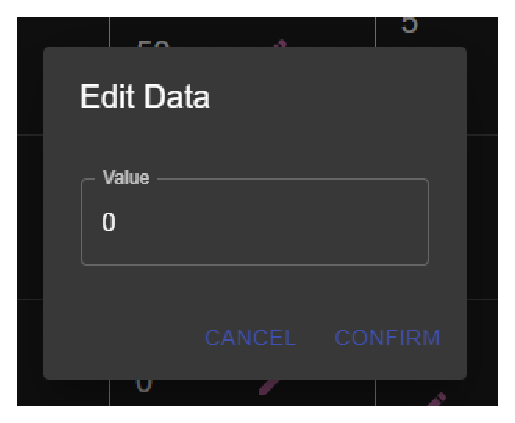
\includegraphics[width=0.4\linewidth]{editextrainfo}
	\caption{Ténylegesen elvégzett adat űrlapja}
	\label{fig:editextrainfo}
\end{figure}

A \ref{fig:cycleclient} ábrán látható egy ciklushoz tartozó edzéstervet tartalmazó oldal. A felső menüsáv alatt a jelenlegi nézetben lévő hétnek a száma található. Alatta bal oldalon egy gomb (Download PDF), amivel le tudjuk tölteni nyomtatható PDF formában a tervet. Az oldal közepén az edzésterv táblázata, napokra felosztva. A tervben a hetek között az egyes gyakorlatok közösek, viszont eltérhetnek súlyban, szériákban, ismétlésben és RPE számban. Az is állandó egy terven belül, hogy hány edzésnapból áll egy hét. Az oldal alján látható kék (vagy szürke, ha nem tudunk abban az irányban hetet váltani), nyíl ikonnal ellátott gomb megnyomásával a hetek között válthatunk. A jobb alsó sarokban lévő mentés ikonra kattintva (amíg nincs el nem mentett módosítás, szürke marad) az összes elvégzett módosítás elmentődik az adatbázisba.

A súly (Weight) oszlopban a ceruza ikonra kattintva a \ref{fig:editweight} ábrán látható űrlap jelenik meg. A bemeneti mezőbe egy nemnegatív és kisebb, mint 10000 értéket írhatunk be. Ezt az értéket a "Confirm" gombbal táblázatba helyezzük.

A "Series", "Repetitions" és "RPE" oszlopokban is megjelennek ceruza ikonok, ezeknél az oszlopoknál a ténylegesen elvégzett értéket adhatjuk meg az adott gyakorlatra, amennyiben az eltérne az edző által kitűzött céltól. Itt csak nem negatív és kisebb, mint 100 értéket adhatunk meg. Az itt rögzített érték a kliens számára edzés naplózási célból, edzője számára pedig mint visszajelzés értendő, ugyanis ő is látni fogja ezeket az adatokat.

\subsection{Chat oldal (kliens)}

\begin{figure}[H]
	\centering
	\includegraphics[width=1\linewidth]{chatclient}
	\caption{Chat oldal (kliens)}
	\label{fig:chatclient}
\end{figure}

A chat oldal a fenti \ref{fig:chatclient} ábrán látható, ahol a kliens felhasználó üzenetet küldhet az edzőjének. A bejelentkezett felhasználó küldött üzenetei mindig a jobb oldalon jelennek meg kék háttérszínnel, míg csevegő társától kapott üzenetek pedig a bal oldalon, szürke színnel. Az üzenetek a jobb alsó sarokban lévő küldés gomb megnyomása, vagy az "ENTER" billentyű lenyomása után azonnal elküldésre kerülnek a másik fél számára, és valós időben meg is jelennek.

\bigskip

Az üzenet hossza nem haladhatja meg a 255 karakterszámot.

\subsection{Profil beállítások (kliens)}

\begin{figure}[H]
	\centering
	\includegraphics[width=1\linewidth]{accountpageclient}
	\caption{Profil beállítások (kliens)}
	\label{fig:accountpageclient}
\end{figure}

Megadott felhasználónév (kevesebb, mint 30 karakter), jelszó megváltoztatására, illetve email értesítések ki/be kapcsolására a \ref{fig:accountpageclient} ábrán látható Profil beállítások oldalon van lehetőség. Bármilyen módosítás elmentéséhez meg kell adnunk a régi jelszavunkat a fiókhoz, amíg ez a mező üres, az űrlapot nem lehet elküldeni.

Az űrlapon a fentieken kívül megtekinthetünk különböző, fiókunkkal kapcsolatos információt, mint: megadott email cím, fiók létrehozásának dátuma, fiókunk típusa. Kliens felhasználók esetén az oldal kiírja edzőnk nevét, valamint a ciklusaink számát.

\subsection{Kezdőlap (edző)}

\begin{figure}[H]
	\centering
	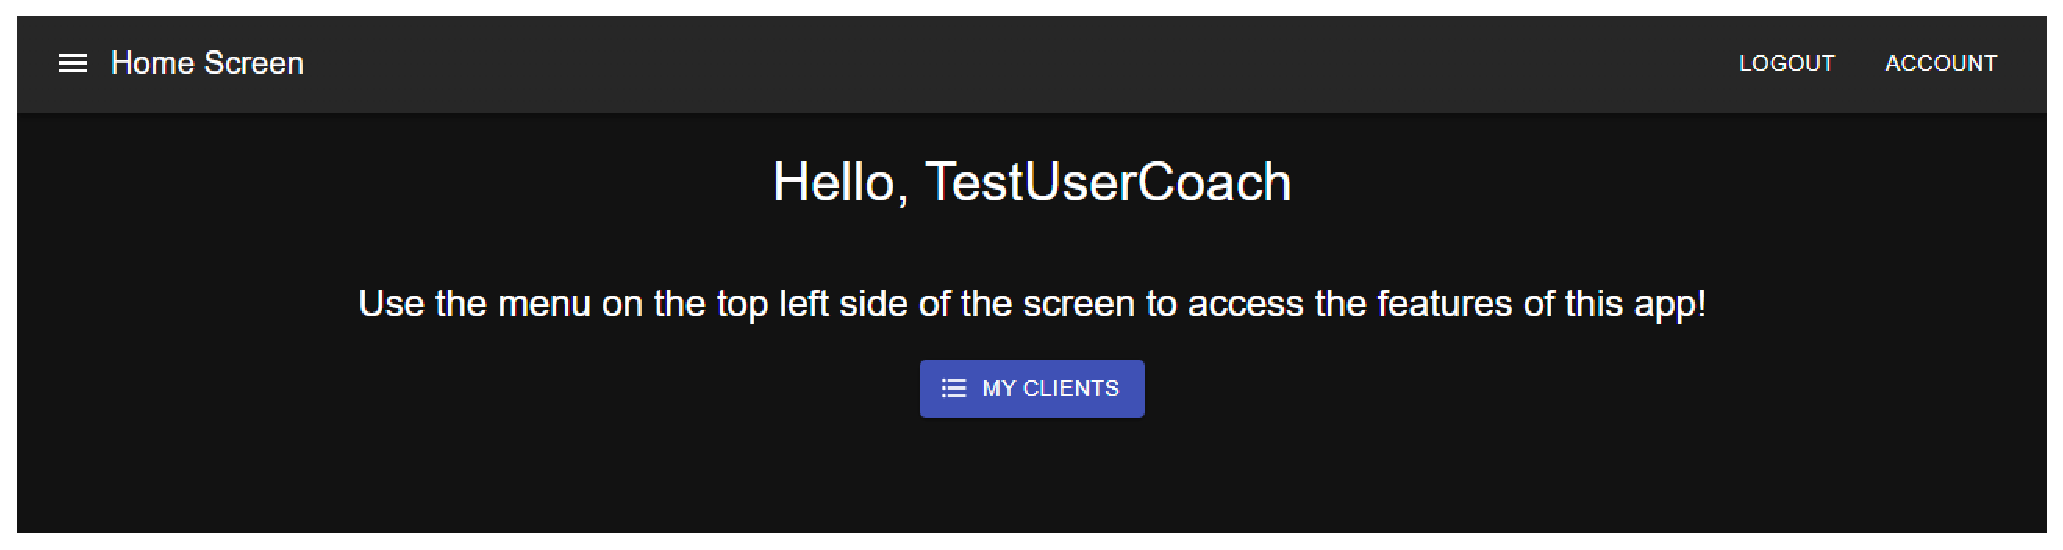
\includegraphics[width=1\linewidth]{kezdolapcoach}
	\caption{Kezdőlap (edző)}
	\label{fig:kezdolapcoach}
\end{figure}

A \ref{fig:kezdolapcoach} ábrán látható kezdőlap az edző jogosultsággal rendelkező fiókok esetén jelenik meg. A kliens fiókok kezdőlapjától csak annyiban tér el, hogy az oldalon található "My Clients" gomb az edző felhasználó klienseinek a listázó oldalára fog továbbítani.

\subsection{Kliensek listzázó oldal (edző)}

\begin{figure}[H]
	\centering
	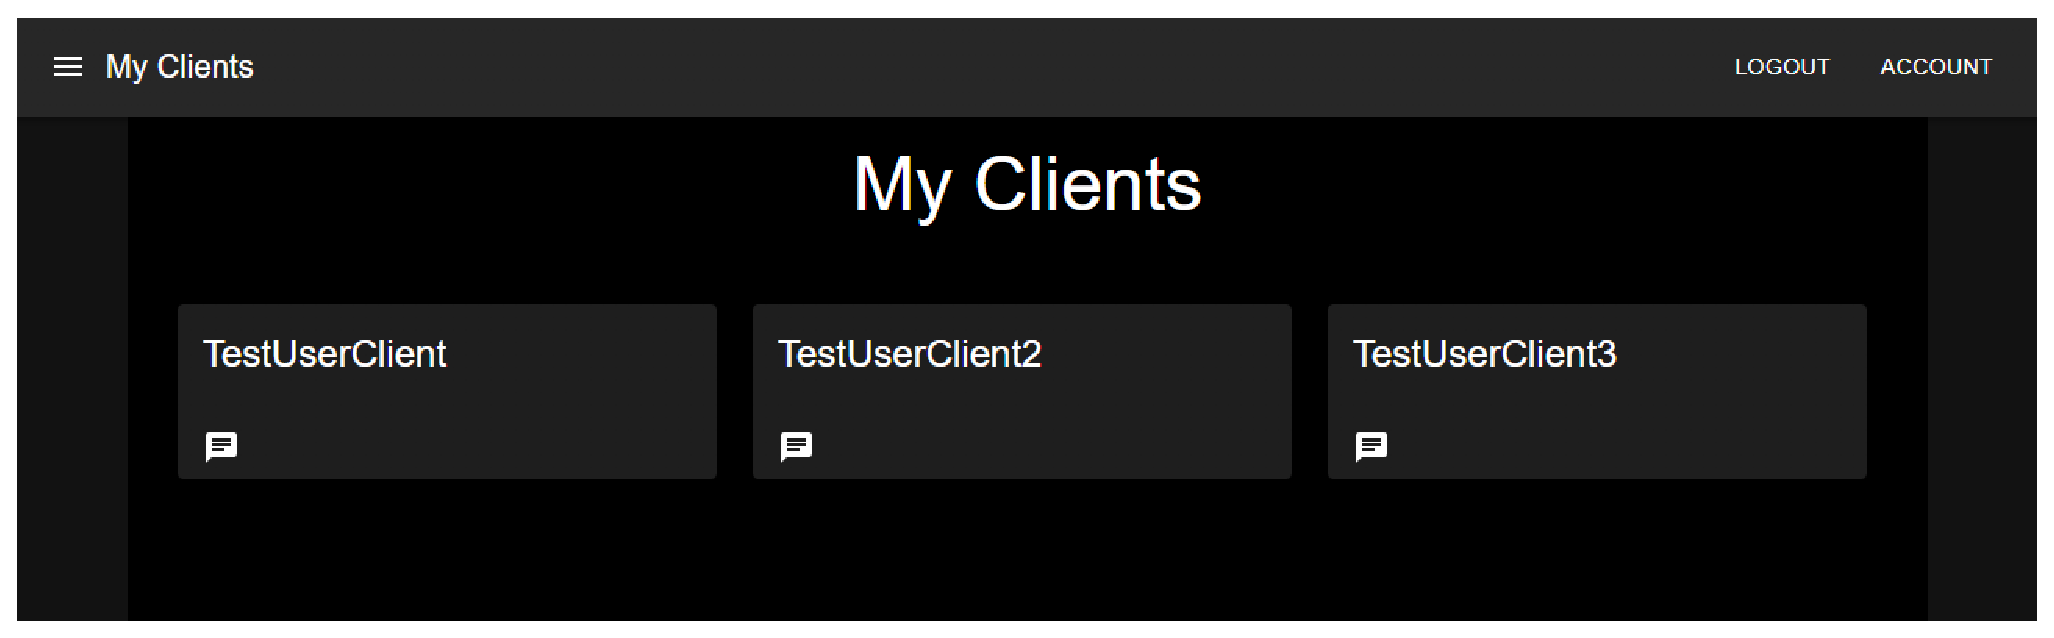
\includegraphics[width=1\linewidth]{clientspage}
	\caption{Kliensek listzázó oldal (edző)}
	\label{fig:clientspage}
\end{figure}

A \ref{fig:clientspage} ábrán megjelenő oldalon edző felhasználóknak a kliensek listázó oldala látható. Itt külön cellákban jelennek meg a felhasználó kliensei, felhasználónév alapján feltüntetve. Egy ilyen cellára kattintva átkerülünk az adott kliens ciklusainak listázó oldalára. A cellákban található egy chat ikon, ezt megnyomva az adott kliensnek tudunk üzeneteket küldeni, hasonlóan a \ref{fig:chatclient} ábrán látható felülethez.

\subsection{Kliens ciklusainak listázó oldala (edző)}

\begin{figure}[H]
	\centering
	\subcaptionbox{Listázó oldal}{
		\includegraphics[width=1\linewidth]{clientpage}}
	\hspace{5pt}
	\subcaptionbox{Ciklus hozzáadása űrlap}{
		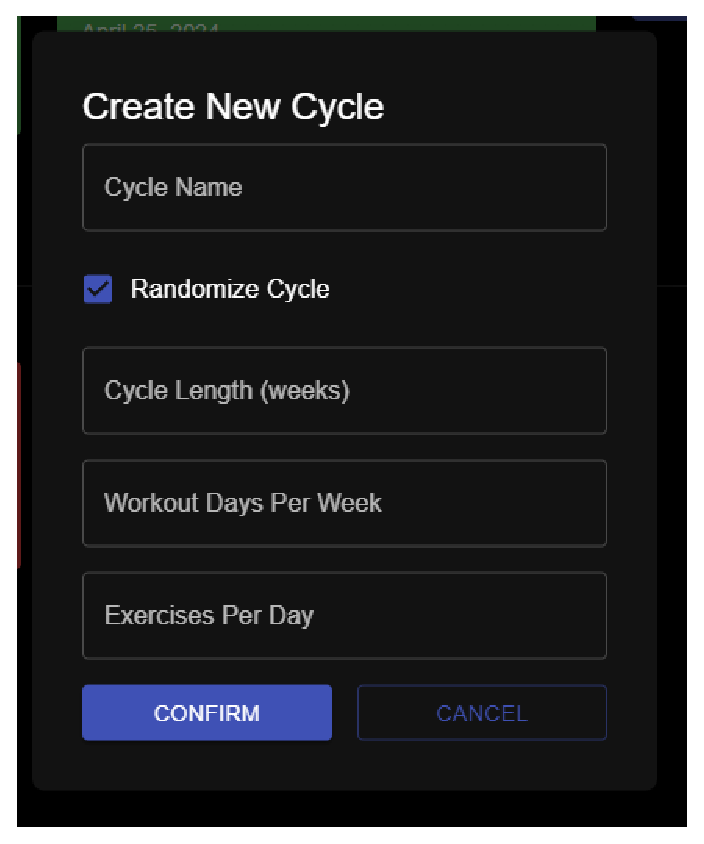
\includegraphics[width=0.45\linewidth]{randomcycle}}
	\caption{Kliens ciklusainak listázó oldala (edző)}
	\label{fig:clientpage}
\end{figure}

Adott kliensünknek a ciklusait megtekinteni, módosítani, törölni, aktív státuszát megváltoztatni, illetve új ciklust létrehozni a \ref{fig:clientpage} ábrán lévő oldalon tudunk. Az oldal felépítése hasonló a kliens nézethez (\ref{fig:cyclesclient}), egy cellára kattintva szintén az adott ciklust tudjuk megtekinteni.

Ha ciklust szeretnénk törölni, a törlés gomb megnyomása után egy felugró ablakban a jóváhagyást követően a ciklus maradandóan törölve lesz az adatbázisból. Az archiválás ikonra kattintva pedig az aktív ciklust inaktívvá, az inaktívat aktívvá tudjuk tenni.

Új ciklus hozzáadása a kék háttérszínű plusz gombbal lehetséges. Ilyenkor megjelenik egy űrlap a képernyőn, ahol válaszhatunk nevet a ciklusnak, illetve opcionálisan tudunk véletlenszerűen generálni a már megírt programok gyakorlatai közül (\ref{fig:clientpage} ábra). Meg kell ilyenkor adnunk, hogy hány hetes legyen a program, mennyi edzésnap legyen hetente, illetve hány darab gyakorlatot szeretnénk naponta.

\subsection{Ciklus/edzésterv oldal (edző)}

\begin{figure}[H]
	\centering
	\includegraphics[width=1\linewidth]{cyclecoach}
	\caption{Ciklus/edzésterv oldal (edző)}
	\label{fig:cyclecoach}
\end{figure}

\begin{figure}[H]
	\centering
	\subcaptionbox{Gyakorlat hozzáadása űrlap}{
		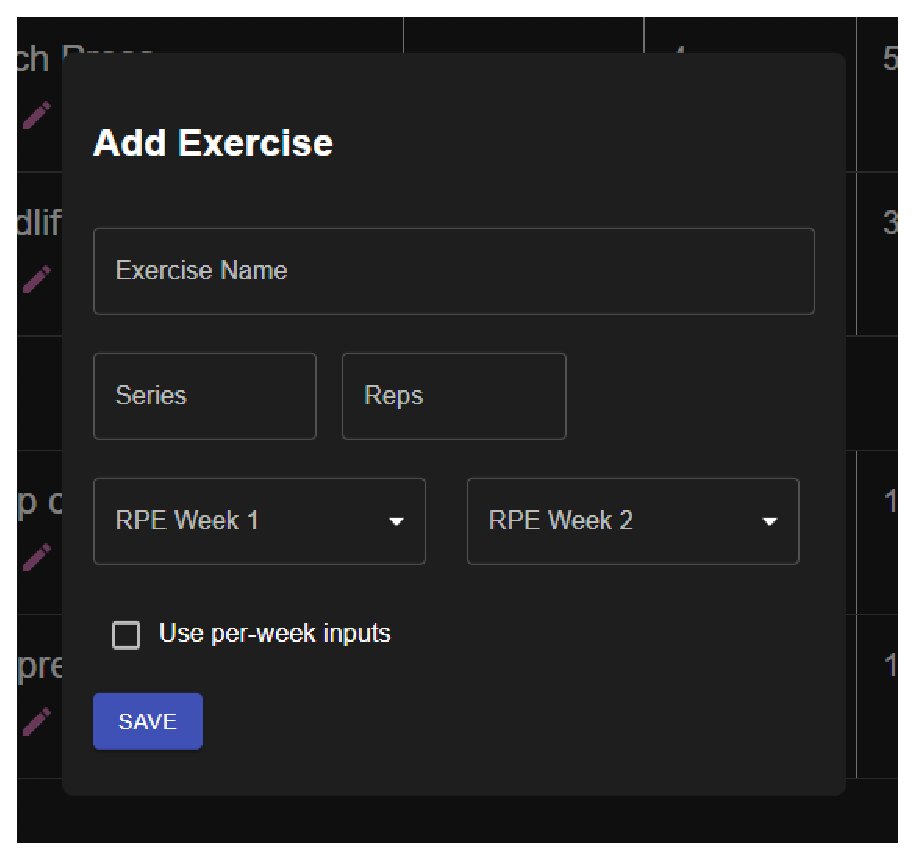
\includegraphics[width=0.45\linewidth]{addexercise}}
	\hspace{5pt}
	\subcaptionbox{Gyakorlat hozzáadása űrlap (hetenkénti bemenet)}{
		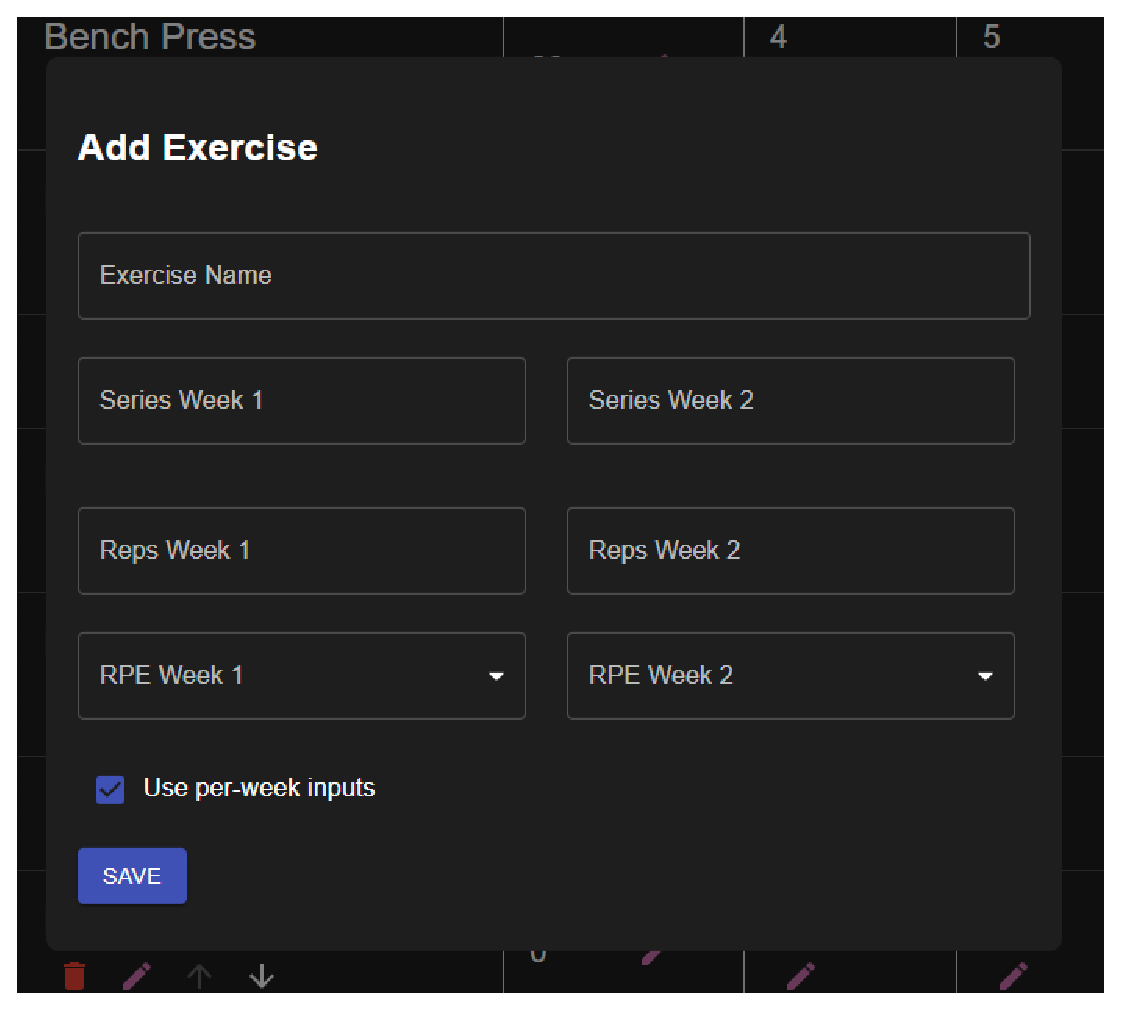
\includegraphics[width=0.45\linewidth]{addexerciseperweek}}
	\caption{Gyakorlat hozzáadása űrlapok}
	\label{fig:addexercise}
\end{figure}

\begin{figure}[H]
	\centering
	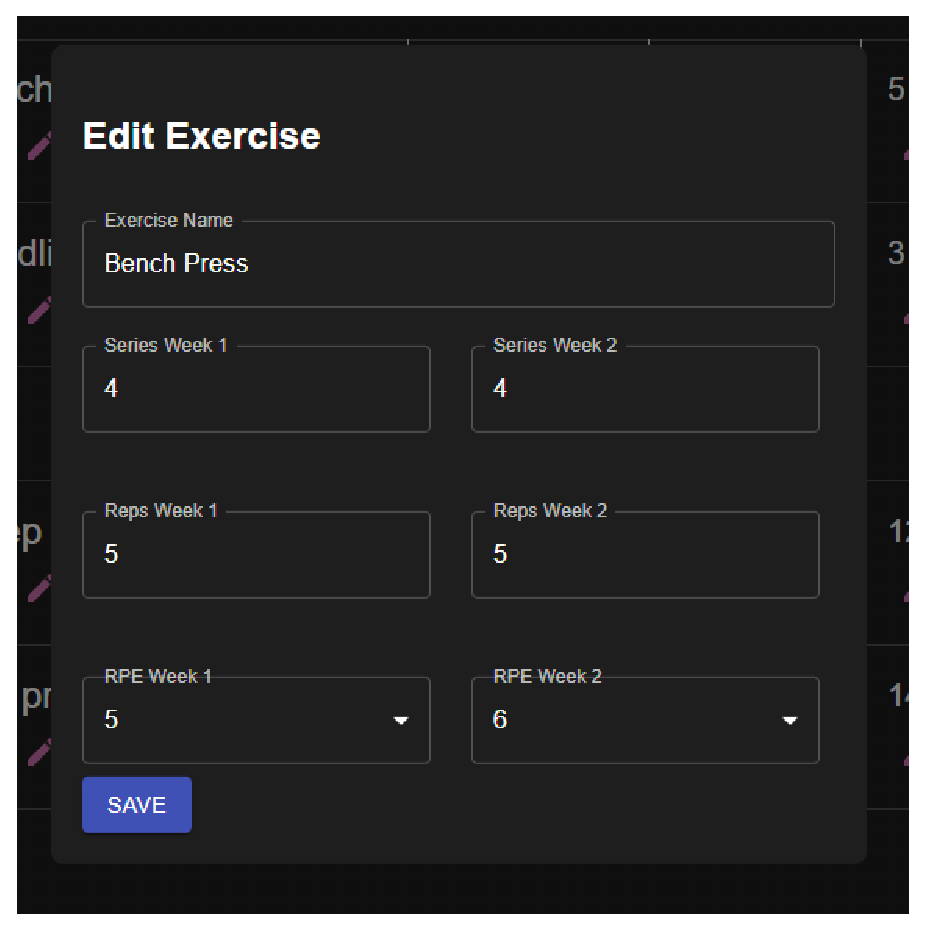
\includegraphics[width=0.6\linewidth]{editexercise}
	\caption{Gyakorlat módosítása űrlap}
	\label{fig:editexercise}
\end{figure}

\begin{figure}[H]
	\centering
	\subcaptionbox{RPE választó}{
		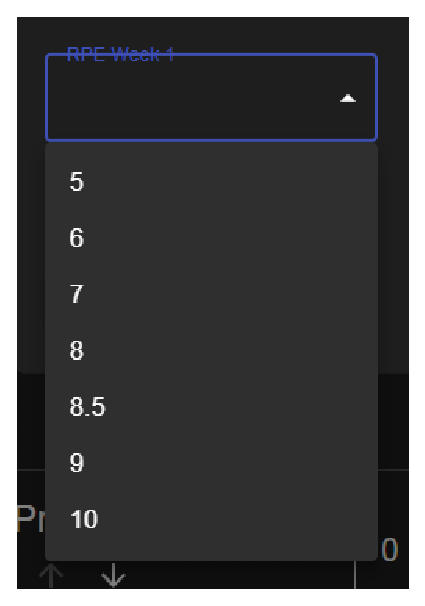
\includegraphics[width=0.3\linewidth]{rpeselector}}
	\hspace{5pt}
	\subcaptionbox{Új hét hozzáadása gomb}{
		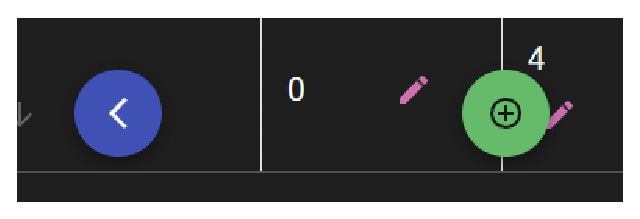
\includegraphics[width=0.3\linewidth]{addnewweek}}
	\caption{Egyéb bemenetek}
	\label{fig:rpeselector}
\end{figure}



Egy edzésterv megjelenítő oldal a \ref{fig:cyclecoach} számú ábrán látható módon jelenik meg. Hasonló a kliens nézethez, kibővítve sok adat módosító funkcióval. A funkciók magyarázata közben a felhasználói felületen látható gombok fentről lefelé vett sorrendjében fogok haladni.

\begin{description}
	\item[Hét törlése:] Az oldal tetején látható törlés ikonnal (hét száma felirat alatt) egy felugró ablak elfogadását követően törölni tudunk egy adott hetet a programból.
	\item[Gyakorlat törlése:] A gyakorlat neve alatt a törlés ikon kitörli a gyakorlatot a programból.
	\item[Gyakorlat módosítása:] A ceruza ikon segítségével gyakorlatokat tudunk módosítani, a módosító űrlapot a \ref{fig:editexercise} ábrán láthatjuk. Változtatni tudjuk a gyakorlat nevét, a szériákat, ismétlések számát és RPE számokat a ciklusban hetenként. A "Save" gomb megnyomásával felülírjuk a régi adatokat az űrlapban megadottakkal. RPE számot a \ref{fig:rpeselector} ábrán látható értékek közül választhatunk.
	Gyakorlat nevének maximum hossza 30 karakter, és minden más adatnak pozitív egész, kisebb mint 100 kritériumoknak megfelelő számnak kell lennie
	\item[Gyakorlat mozgatása:] A nyíl ikonokkal a gyakorlatot tudjuk pakolni egy cellával feljebb vagy lejjebb az adott napon belül. Ez például akkor lehet fontos, ha előrébb szeretnénk vinni egy nehezebb gyakorlatot, amelyet majd könnyebbek követnek.
	\item[Súly módosítása:] Ha edzőként meg szeretnénk adni ajánlott súly mennyiséget egy gyakorlathoz, azt ezzel a gombbal megtehetjük (felülete és hatása megegyezik a \ref{fig:cycleclient} ábráról elmondottakkal).
	\item[Sorozatok/ismétlések/RPE módosítás:] A "Gyakorlat szerkesztése" űrlapon kívül az adott oszlophoz tartozó ceruza ikonra kattintva is meg tudjuk változtatni a gyakorlathoz rögzített adatokat, az űrlap megjelenése azonos a \ref{fig:editextrainfo} ábrával.
	\item[Nap törlése:] A nap száma melletti törlés gombra kattimtva az adott nap, összes gyakorlatával együtt törlésre kerül.
	\item[Gyakorlat hozzáadása:] Az adott naphoz tartozó gyakorlatok listája alatt egy újabb sorban látható egy hozzáadás gomb. Ennek megnyomásával felugrik a \ref{fig:addexercise} ábrán látható ablak. Meg kell adnunk a  gyakorlat nevét, illetve különböző információkat róla. A "Use per-week inputs" gombbal ki-be kapcsolhatjuk a hetenkénti bemenetet a szériák és ismétlések számára. Ezt azt jelenti, ha kikapcsoljuk a funkciót, a két bemeneten megadott szám hetenként meg fog egyezni a gyakorlaton. Ha be van kapcsolva, variálni tudjuk a hetek között az értékeket. Ennek célja, hogy egyszerűbbé tegye a sok gyakorlat rögzítését az edző felhasználóknak, ugyanis ciklusokon belül ezek az értékek általában megegyeznek. 
	Gyakorlat nevének maximum hossza 30 karakter, és minden más adatnak pozitív egész, kisebb mint 100 kritériumoknak megfelelő számnak kell lennie
	\item[Nap hozzáadása:] A "Day" oszlop alján lévő plusz gombbal az edzéstervhez extra napot adhatunk.
	\item[Hetek közötti lapozás / mentés gomb:]  A nyilakkal hetek között válthatunk, a mentés gombbal pedig véglegesítjük a változtatásokat.
	\item[Új hét hozzáadása:] Ha el lapozunk a programban lévő utolsó hétre, a jobb oldali nyíl gomb egy plusz ikonra változik. Ennek megnyomásával és a felugró ablak elfogadásával új hét adódik a ciklushoz. 
\end{description}

Fontos megjegyezni, hogy ezen az oldalon történt változtatások véglegesítéséhez rá kell kattintani a mentés gombra, különben elvesznek.

\subsection{Profil beállítások (edző)}

\begin{figure}[H]
	\centering
	\includegraphics[width=1\linewidth]{accountpagecoach}
	\caption{Profil beállítások (edző)}
	\label{fig:accountpagecoach}
\end{figure}

Az edzői fiókhoz tartozó profil beállítások a \ref{fig:accountpagecoach} ábrán láthatóak. A beállítások nagy része azonos a \ref{fig:accountpageclient} ábrán láthatóakkal, kivéve az "Additional Information" fül alatt lévőket. Itt információt kapunk a mi (edző) azonosító kódunkról, amelyet klienseink regisztráció során meg tudnak adni. Ezen kívül a klienseink számát is megtekinthetjük.

\subsection{Felhasználók listája (adminisztrátor)}

\begin{figure}[H]
	\centering
	\includegraphics[width=1\linewidth]{manageusers}
	\caption{Felhasználók listája (adminisztrátor)}
	\label{fig:manageusers}
\end{figure}

A fenti \ref{fig:manageusers} ábrán az adminisztrátor felület látható. Ez a felhasználók kezelésére szolgál. Információkat láthatunk a fiók típusárol, az egyéni azonosítójukról, valamint a csatlakozási dátum is fel van tűntetve. Felhasználói fiókokat törölhetünk a "Delete User" gombbal, klienseket rendelhetünk edzőkhöz az "Add Client" gombbal, illetve ha lenyitjuk a "Clients" listát egy edző felhasználónak, klienseket is ki tudunk törölni az adott edzőhöz tartozó listából. Az oldalon a felül található menü használatával a különböző típusú fiókokra szűrhetjük a nézetet.

\pagebreak

\section{Megjelenő üzenetek}

A program használata során számos üzenet megjelenhet. Közöttük vannak hibaüzenetek, és visszaigazolás jellegűek. Típustól függetlenül az oldal bal alsó sarkában láthatóak, zöld vagy piros színnel, rendre ha visszaigazolás vagy hiba jellegűek.

\subsection{Visszaigazoló üzenetek}

\begin{figure}[htbp]
	\centering
	\begin{subfigure}[b]{0.3\textwidth}
			\centering
			
\includegraphics[width=\textwidth]{deleteclient}
			\caption{Kliens törlése}
			\label{fig:deleteclient}
	\end{subfigure}
	\hfill
	\begin{subfigure}[b]{0.3\textwidth}
			\centering
			
\includegraphics[width=\textwidth]{addclient}
			\caption{Kliens hozzáadása}
			\label{fig:addclient}
	\end{subfigure}
	\hfill
	\begin{subfigure}[b]{0.3\textwidth}
			\centering
			\includegraphics[width=\textwidth]{deleteuser}
			\caption{Kliens törlése}
			\label{fig:deleteuser}
	\end{subfigure}
	
	\medskip
	
	\begin{subfigure}[b]{0.3\textwidth}
			\centering
			\includegraphics[width=\textwidth]{weekdelete}
			\caption{Hét törlése}
			\label{fig:weekdelete}
	\end{subfigure}
	\hfill
	\begin{subfigure}[b]{0.3\textwidth}
			\centering
			\includegraphics[width=\textwidth]{exerciseedit}
			\caption{Gyakorlat módosítása}
			\label{fig:exerciseedit}
	\end{subfigure}
	\hfill
	\begin{subfigure}[b]{0.3\textwidth}
			\centering
			
\includegraphics[width=\textwidth]{exercisedelete}
			\caption{Gyakorlat törlése}
			\label{fig:exercisedelete}
	\end{subfigure}
	
	\medskip
	
	\begin{subfigure}[b]{0.3\textwidth}
			\centering
			
\includegraphics[width=\textwidth]{exerciseadd}
			\caption{Új gyakorlat hozzáadása}
			\label{fig:exerciseadd}
	\end{subfigure}
	\hfill
	\begin{subfigure}[b]{0.3\textwidth}
			\centering
			\includegraphics[width=\textwidth]{deleteday}
			\caption{Nap törlése}
			\label{fig:deleteday}
	\end{subfigure}
	\hfill
	\begin{subfigure}[b]{0.3\textwidth}
			\centering
			\includegraphics[width=\textwidth]{adday}
			\caption{Nap hozzáadása}
			\label{fig:adday}
	\end{subfigure}
	
	\medskip
	
	\begin{subfigure}[b]{0.3\textwidth}
			\centering
			
\includegraphics[width=\textwidth]{cycledeactivate}
			\caption{Ciklus deaktiválása}
			\label{fig:cycledeactivate}
	\end{subfigure}
	\hfill
	\begin{subfigure}[b]{0.3\textwidth}
			\centering
			
\includegraphics[width=\textwidth]{cycleactive}
			\caption{Ciklus aktiválása}
			\label{fig:cycleactive}
	\end{subfigure}
	\hfill
	\begin{subfigure}[b]{0.3\textwidth}
			\centering
			\includegraphics[width=\textwidth]{registermessage}
			\caption{Regisztráció}
			\label{fig:registermessage}
	\end{subfigure}
	
	\medskip
	
	\begin{subfigure}[b]{0.3\textwidth}
			\centering
			\includegraphics[width=\textwidth]{accountpagesave}
			\caption{Profil adatok frissítése}
			\label{fig:accountpagesave}
	\end{subfigure}
	\hfill
	\begin{subfigure}[b]{0.3\textwidth}
			\centering
			
\includegraphics[width=\textwidth]{cyclesaved}
			\caption{Ciklus elmentése}
			\label{fig:cyclesaved}
	\end{subfigure}
	\hfill
	\begin{subfigure}[b]{0.3\textwidth}
			\centering
			\includegraphics[width=\textwidth]{loggedinmessage}
			\caption{Bejelentkezés}
			\label{fig:loggedinmessage}
	\end{subfigure}
	
	\caption{Visszaigazoló üzenetek}
	\label{fig:visszaigazolo}
\end{figure}

Ezek a lehetséges visszaigazoló üzenetek, amelyekkel a program használata közben találkozhatunk (\ref{fig:visszaigazolo}). Céljuk csupán egy gyors visszajelzést adni a felhasználónak, hogy a kért művelet valóban elvégződött-e.

\pagebreak

\subsection{Hibaüzenetek}

\begin{figure}[htbp]
	\centering
	\begin{subfigure}[b]{0.3\textwidth}
		\centering
		
\includegraphics[width=\textwidth]{errorlogin}
		\caption{Rossz adatok bejelentkezéskor}
		\label{fig:errorlogin}
	\end{subfigure}
	\hfill
	\begin{subfigure}[b]{0.3\textwidth}
		\centering
		
\includegraphics[width=\textwidth]{internalerror}
		\caption{Szerver hiba}
		\label{fig:internalerror}
	\end{subfigure}
	\hfill
	\begin{subfigure}[b]{0.3\textwidth}
		\centering
		
\includegraphics[width=\textwidth]{errorcoachid}
		\caption{Rossz edző azonosító megadása regisztrációkor}
		\label{fig:errorcoachid}
	\end{subfigure}
	\hfill
	\begin{subfigure}[b]{0.4\textwidth}
		\centering
		
\includegraphics[width=\textwidth]{errornotloggedin}
		\caption{Nincs jogosultság az oldal megnyitásához}
		\label{fig:errornotloggedin}
	\end{subfigure}
	
	\caption{Hibaüzenetek}
	\label{fig:hiba}
\end{figure}

A \ref{fig:hiba} ábrán látható néhány lehetséges hibaüzenet. Ha egy ilyet látunk, a kért művelet nem ment végbe, így újra kell próbálni azt. A "Szerver hiba" üzenet felléphet, ha nincsen kapcsolatunk a szerverhez, vagy egyéb más szerveroldali hiba fellépése esetén. Ha lehetséges, a szerver is képes részletesebb üzenetet küldeni a hiba okáról.

\subsection{Űrlapon megjelenő hibaüzenetek}

\begin{figure}[H]
	\centering
	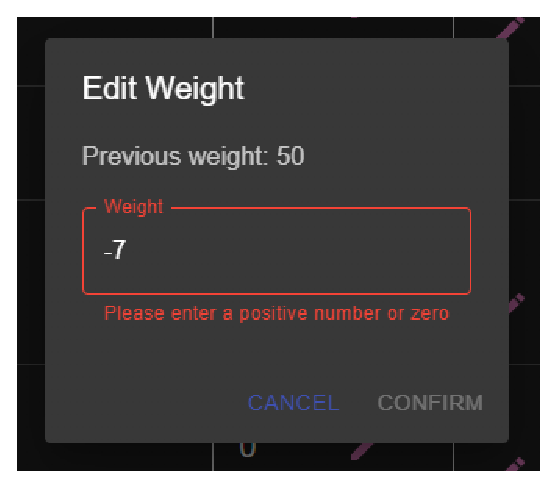
\includegraphics[width=0.5\linewidth]{editweighterror}
	\caption{Űrlap hibaüzenet}
	\label{fig:editweighterror}
\end{figure}

A ciklus oldalon (\ref{fig:cycleclient} / \ref{fig:cyclecoach}) található űrlapokon a fenti \ref{fig:editweighterror} ábrához hasonló üzenetbe ütközünk, ha a beírt szám negatív. Ilyenkor nem tudjuk elmenteni az adatot, a küldés gomb inaktívvá válik.